\chapter{Action Recognition}
\section{Introduction}
\label{sec:actreg:intro}

Recognising human actions from videos has been widely studied for practical applications such as human-computer interfaces, digital entertainment, visual surveillance and automatic video indexing. Despite popularity of the topic in computer vision research, some issues still remain unsolved for realising its potentials:
\begin{itemize}

\item While \emph{time efficiency} is of vital importance in real-world action recognition systems, current methods seldom take the computational complexity into full consideration. State-of-the-art algorithms have reported satisfactory accuracies on standard human action data sets. They, however, utilise complex algorithms to improve accuracies at the expense of increasing overall computational time.

\item Action classification with \emph{a short response time} is beneficial to continuous recognition in human-computer interaction. Typically, an class label is assigned after the entire query video is analysed, or a large lookahead is required to collect sufficient features. In fact, as suggested by \cite{Schindler2008}, actions can be recognised from very short sequences called the ``snippets''.

\item {\em Structural information} is a useful cue for action recognition. A standard ``bag of words'' model has proven effective for action recognition owing to its rich description power of local appearance information and its inherent benefits to cope with scale changes, translation and cluttered backgrounds. It, however, does not consider structural relationship among features. 

\end{itemize}

Addressing the aforementioned challenges, we present a novel method for human action recognition.
The goal of this work is to design a very fast but equally effective action recogniser.
In the method we intend to exploit as much information as possible in a relatively short video sequence, local appearance and structural information are integrated adaptively.
The major contributions include the followings.

Firstly, inspired by the work of Shotton \etal{Shotton2008}, we extend the use of semantic texton forests from 2D image segmentation to spatiotemporal analysis. STFs are ensembles of random decision trees that translate interest points into visual codewords. In our method, STF performs directly on video pixels without computing expensive local descriptors and efficiently generates codewords. As well as being faster than a traditional flat codebook such as k-means clustering, STF achieves high effectiveness comparable to that of existing approaches.
As far as we are aware, this is the first method that uses STF in action recognition studies.

Secondly, the method combines structure and local appearance information based on STF. This results into a richer description of human actions, hence actions can be classified in very short video sequences. Building on the work of Ryoo and Aggarwal{Ryoo2009}, we introduce the multi-pyramidal spatiotemporal relationship match (MpSRM). In the original approach, structural information of spatiotemporal features are matched linearly. Quantization errors affect the robustness of recognition results. Taking the inherent benefit of the hierarchical structure of semantic texture forest, a pyramidal match kernel \cite{Grauman2005} is employed to alleviate the quantization problem.
A fast and effective classifier, namely k-means forest classifier, is also proposed.

Lastly, several techniques are employed to improve the recognition speed and accuracy. A novel spatiotemporal interest point detector, called V-FAST, is designed based on the FAST 2D corners{Rosten2006}. The recognition accuracy is improved by adaptively combining MpSRM and the bag of semantic texton (BOST) method \cite{Shotton2008}.

The rest of the paper is structured as follows: In section \ref{sec:relatedwork}, related work are reviewed and, in section \ref{sec:overview}-\ref{sec:combine}, the proposed methods are detailed. Evaluation results are reported and discussed in Section \ref{sec:experiments} and the conclusion is drawn in Section \ref{sec:discussion}.


\section{Related Work}
\label{sec:relatedwork}
State-of-the-art action recognition methods have shown the effectiveness of local appearance-based features, as a ``bag of words'' model is especially popular in the literature \cite{Dollar2005, Riemenschneider2009, Niebles2008, Schuldt2004, Wong2007}. A codebook is learned to quantise input features into visual codewords. Classification is then performed on histograms of codewords. Generally, a large codebook is required to obtain a high recognition accuracy, yet an oversized codebook leads to high quantisation errors and overfitting. K-means clustering is a widely adopted algorithm in codebook learning. Feature quantization by a large flat codebook such as k-means is, however, computationally heavy. Therefore, tree-based codebooks have been studied to increase the efficiency of feature quantisation. 
%Since Moosmann \etal{MoosmannNIPS2006}, random forest has been increasingly popular as a powerful discriminative codebook in many tasks e.g. image classification and segmentation \cite{shottonCVPR2008}, owing to its good generalisation and speed. 
Since Moosmann \etal \cite{Moosmann2007}, random forests have been increasingly used in many tasks \eg image classification and segmentation \cite{Shotton2008}, owing to its good generalisation and efficiency. Similarly, Oshin \etal \cite{Oshin2009} recognise actions by analysing the distribution of interest points by random ferns. Lin \etal \cite{Lin2009} used a prototype tree to encode holistic motion-shapes descriptors. Mikolajczyk and Uemura \cite{Mikolajczyk2008} build clustering trees from the centroids computed from k-means algorithm. 
%Using a tree structure makes the quantisation process efficient, however, expensive features and classifier used in{linICCV2009,mikolajczykCVPR2008} make the overall process still heavy.
Hierarchical codebooks enable fast feature quantisations, but the expensive features and classifiers used in{Lin2009,Mikolajczyk2008} make the overall processes still heavy.

Standard bag of words models contain only local appearance information. While structural context could be useful in describing some action classes, it is often omitted in current action recognition methods.
On the other hand, some studies{Gorelick2007, Fathi2008, Lin2009, Kim2007} have implied that structural or holistic features can be as effective as local features.
Several recent studies have attempted to augment structural information into local appearance features. Scovanner \etal \cite{Scovanner2007} employ a two-dimensional histogram to describe the feature co-occurrences. Savarese \etal \cite{Savarese2008} propose ``correlograms'' to measure the similarity of actions globally. Wong \etal \cite{Wong2007} present the pLSA-ISM model, which is an extension of a probabilistic model pLSA with augmented spatial information. 
Tran and Sorokin \cite{Tran2008} and Zhang \etal \cite{Zhang2008} capture structural information directly by using a global shape descriptor.
Since these methods \cite{Wong2007,Tran2008, Zhang2008} encode the hosllistic structures with respect to a reference position \eg a center of ROI (region of interests), they require manual segmentation and computationally-demanding detection of ROI in training and testing respectively. 
However, the structural relationship between among individual features are not fully utilised in these techniques.
Most recently, Ryoo and Aggarwal{Ryoo2009} propose the spatiotemporal relationship match (SRM) which represents structures by a set of pairwise spatiotemporal association rules. Kovashka and Grauman \cite{Kovashka2010} exploit structural information by learning an optimal neighbourhood measure on interest points. Despite of the high accuracies reported, speed and quantisation error are the major issues because flat k-means codebooks are used.

The pyramid match kernel (PMK){Grauman2005} is widely used in recent image-based object detection and matching studies. PMK exploits multi-resolution histograms. Similar points that do not match at fine resolutions have the chance to match at lower resolutions. Hence, PMK reduces quantisation errors and enhances robustness. Liu and Shah \cite{Liu2008} matched interest points in multiple resolutions using PMK and reported improved results, however the features are only matched spatially but not semantically.

Design of interest point detector/descriptor and classifiers also plays an essential role. 
%Just to name a few, Laptev and Lindeberg{laptevICCV2003} and Dollar \etal \cite{dollarPETS2005} propose interest points detector which are the extensions of 2D Harris corners. These interest point detector are widely adopted in existing approaches.
Just to name a few, the detectors designed by Laptev and \cite{Laptev2005} and Dollar \etal \cite{Dollar2005} are commonly adopted in most existing methods. Both of them are the extensions of the two-dimensional Harris corner.
Wong and Cipolla{Wong2007a} extract interest points using global information.
Oikonomopoulos \etal{Oikonomopoulos2005} compute spatiotemporal saliency by measuring the entropy within a spherical neighbourhood.
To describe interest points, histogram of gradients (HOG) and optical flow are popular among earlier approaches \cite{Dollar2005, Niebles2008, Schuldt2004}. Scovanner \etal \cite{Scovanner2007} proposed a three-dimensional version of Lowe's popular SIFT descriptor \cite{Lowe2004}. Willems \etal \cite{Willems2009} used an extended SURF descriptor for action recognition.
Some common classifiers used in action recognition include K-NN classifiers, support vector machines and boosting, which are complex to attain a sufficient real-time performance.

With increasing interests in practical applications, real-time action recognition algorithms have attracted new attentions. For instance, Yeffet and Wolf \cite{Yeffet2009} utilise dense local trinary patterns with a linear SVM classifier. Gilbert \etal \cite{Gilbert2009} propose a fast multi-action recognition algorithm by finding reoccurring patterns on dense 2D Harris corners by a data-mining algorithm.
Patron-Perez and Reid \cite{Patron2007} designed a probabilistic classifier that recognise actions continuously with a sliding window. 
Bregonzio \etal \cite{Bregonzio2009} consider actions as clouds of points, efficient classification is done by analysing histogram of point clusters. Although real-time performances have been reported by these methods, their computation bottlenecks in visual codebook have not yet addressed. 
Some methods require a prior segmentation or a long sequence for classification, rendering these methods efficient but not responsive. 

\section{Overview of the proposed method}
\label{sec:overview}
An overview of the proposed approach is illustrated in figure \ref{img:flow}. Spaiotemporal interest points are first localised by the proposed V-FAST detector. Visual codewords are generated from the interest points by a semantic texton forest. Using pairwise codewords and their spatiotemporal associations, histograms that capture both local-appearance and structural information are constructed. Classification is performed efficiently using a hierarchical k-means algorithm with pyramid match kernels. The proposed method is adaptively combined with the prior-art that uses the bag of semantic texton (BOST) and random forest classifier to further improve the recognition accuracy.
The proposed recognition framework is flexible. Depending on the application, simple spatiotemporal volumes can be replaced by other local features, such as HOG or tracked trajectories.

\begin{figure}
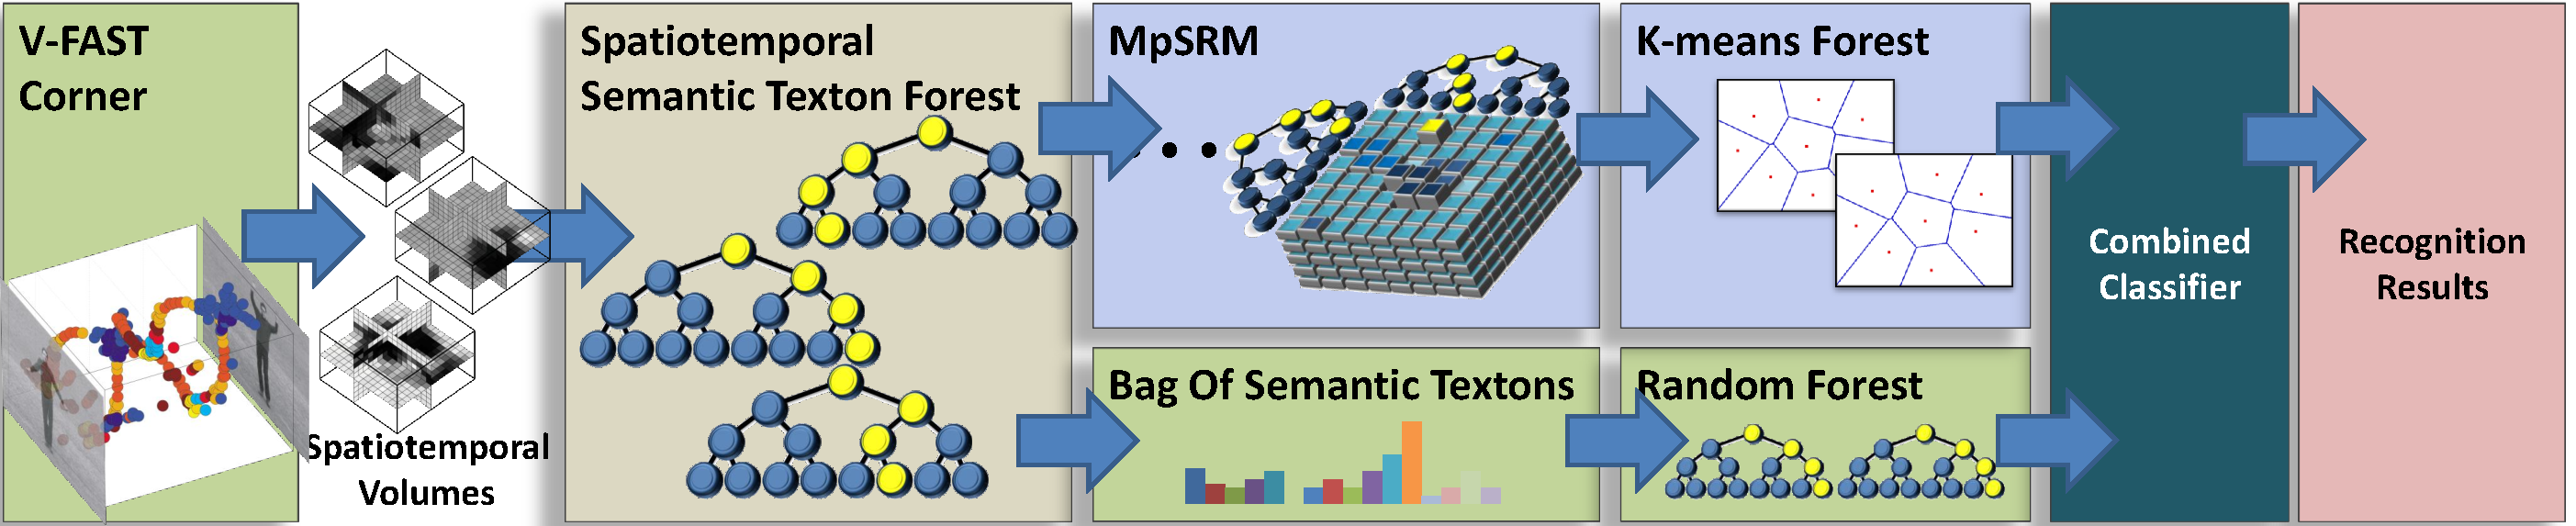
\includegraphics[width=1.0\linewidth]{fig/actreg/fig1_new.pdf}%flow.png}
\caption{Overview of the proposed approach}
\label{img:flow}
\end{figure}

\section{V-FAST Interest Point Detector}
\label{sec:fastest}
The V-FAST (Video FAST) interest point is an extended version of the two-dimensional FAST corner \cite{Rosten2006} to the spatiotemporal domain. It considers pixels in three orthogonal Bresenham circles with radius $r$ on $XY$, $YT$ and $XT$ planes. Similar to FAST, saliency is detected on a plane if there exists $n$ contiguous pixels on the circle which are all brighter than a reference pixel $p(x,y,t)$ plus a threshold $t$, or all darker than $p(x,y,t)-t$. An interest point is detected when the reference pixel shows both spatial ($XY$-plane) and temporal ($XT$-plane or $YT$-plane) saliency. The V-FAST detector gives a denser set of interest points, which enables accurate classification from relatively short sequences. Figure \ref{img:fastest} illustrates how interest points are detected using a 42-pixel V-FAST interest point detector with $r = 3$.
\vspace{-2mm}
\begin{figure}[h]
\centering
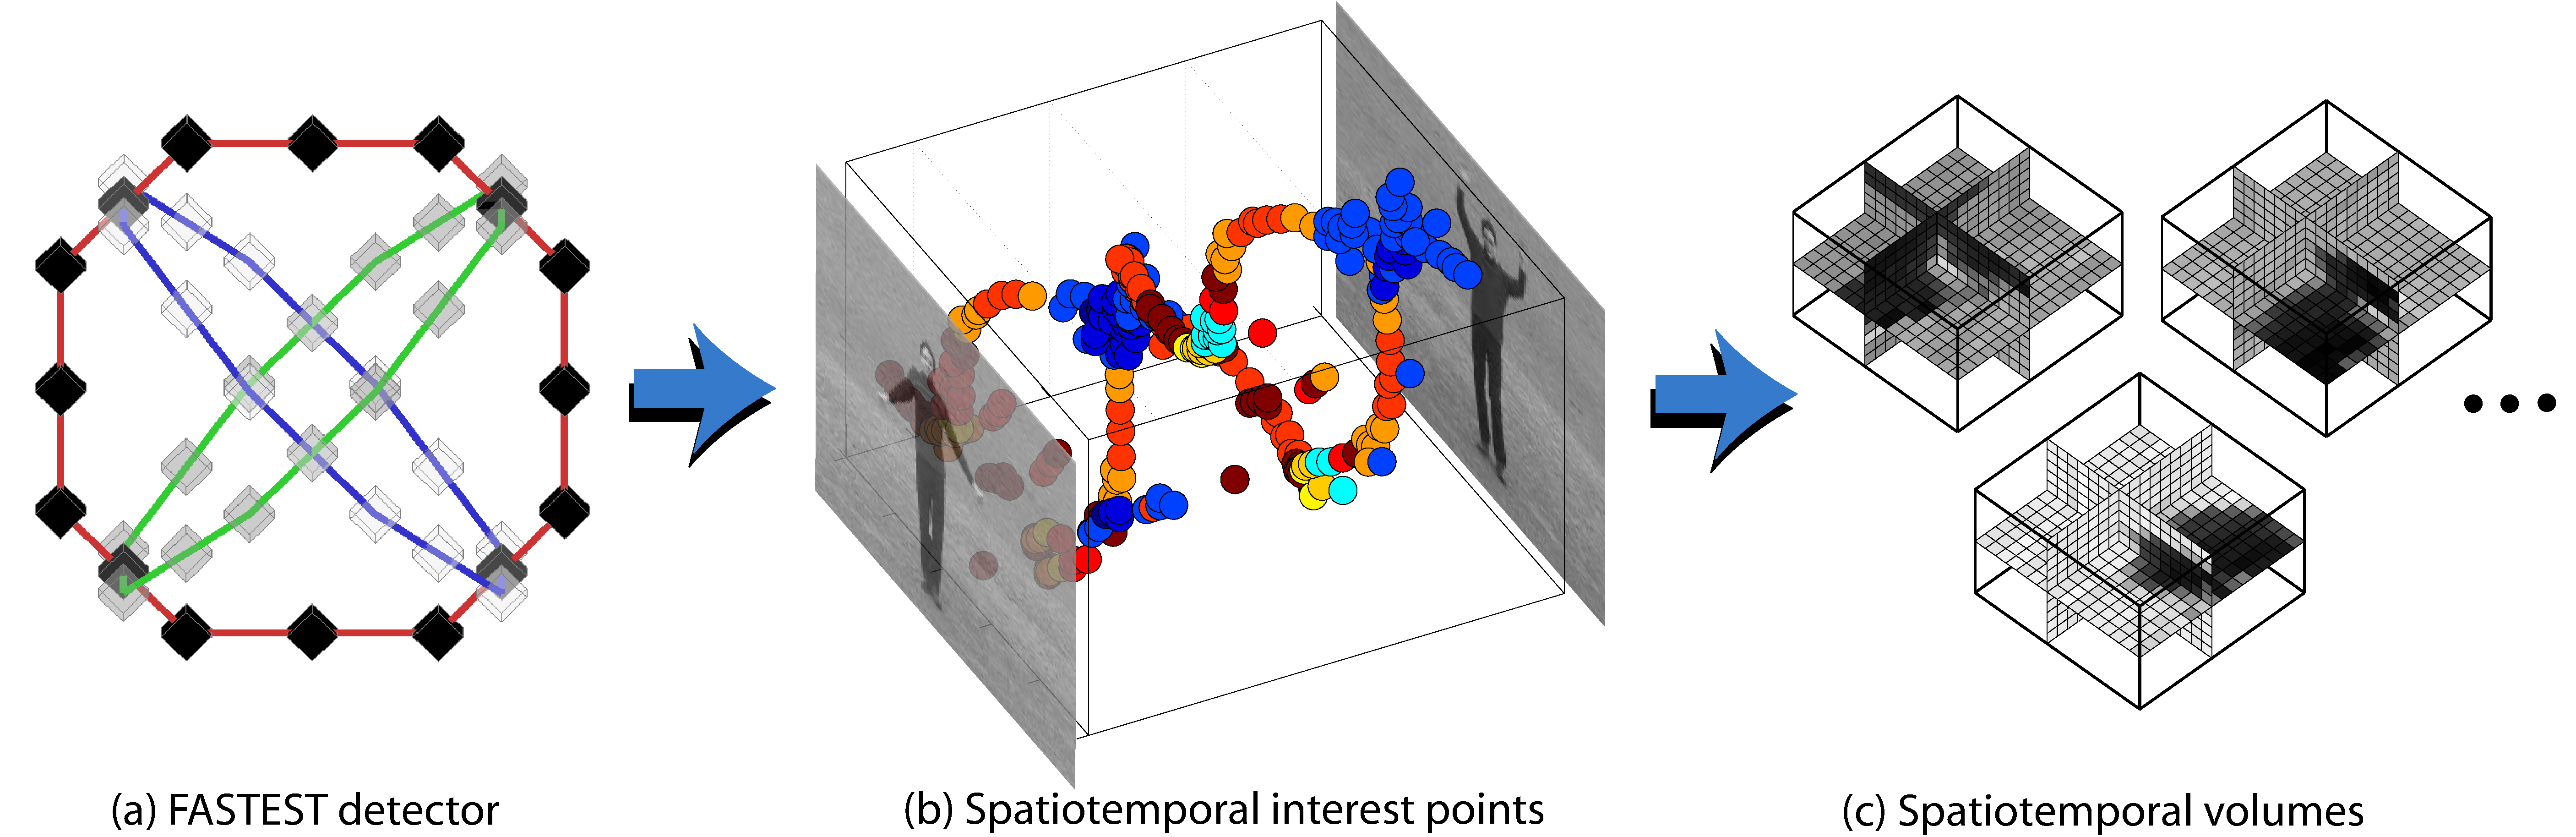
\includegraphics[width=0.8\linewidth]{fig/actreg/fig2_tot.pdf}%fastest.png}
\caption{Spatiotemporal interest points localised by the proposed V-FAST detector}
\label{img:fastest}
\end{figure}\vspace{-5mm}

\section{Spatiotemporal Semantic Texton Forest}
\label{sec:stf}
The semantic texton forest{Shotton2008} is an ensemble of randomised decision trees which textonise input video patches into semantic textons. It is extremely fast to evaluate, since only a small number of simple features is used to traverse the trees. It is also a powerful discriminative codebook composed of multiple decision trees. Figure \ref{img:stf} illustrates how visual codewords are generated using the spatiotemporal semantic texton forest in the proposed method. It acts on small spatiotemporal volumes $p(x,y,t)$, which are localised around the detected interest points from input videos. The training process of STF is similar to that of random forest. At each split node, a number of candidate split functions are generated randomly, the one that maximises the information gain is chosen. The split functions in this work are defined as the weighted differences of two pixels from the input space-time patches: 
\begin{equation}
\mathit{f}(p) = w_1 \cdot p(x_1,y_2,t_1) - w_2 \cdot p(x_2,y_2,t_2) > threshold
\end{equation}
Features are passed down the $M$ trees. Hence, a STF codebook has a size of $L=\sum_m^M L_m$  where $L_m$ represents the number of leaf nodes i.e. codewords in $m$-th tree. Figure \ref{img:stf} (right) shows the two codewords generated with respect to the example split function.
\begin{figure}
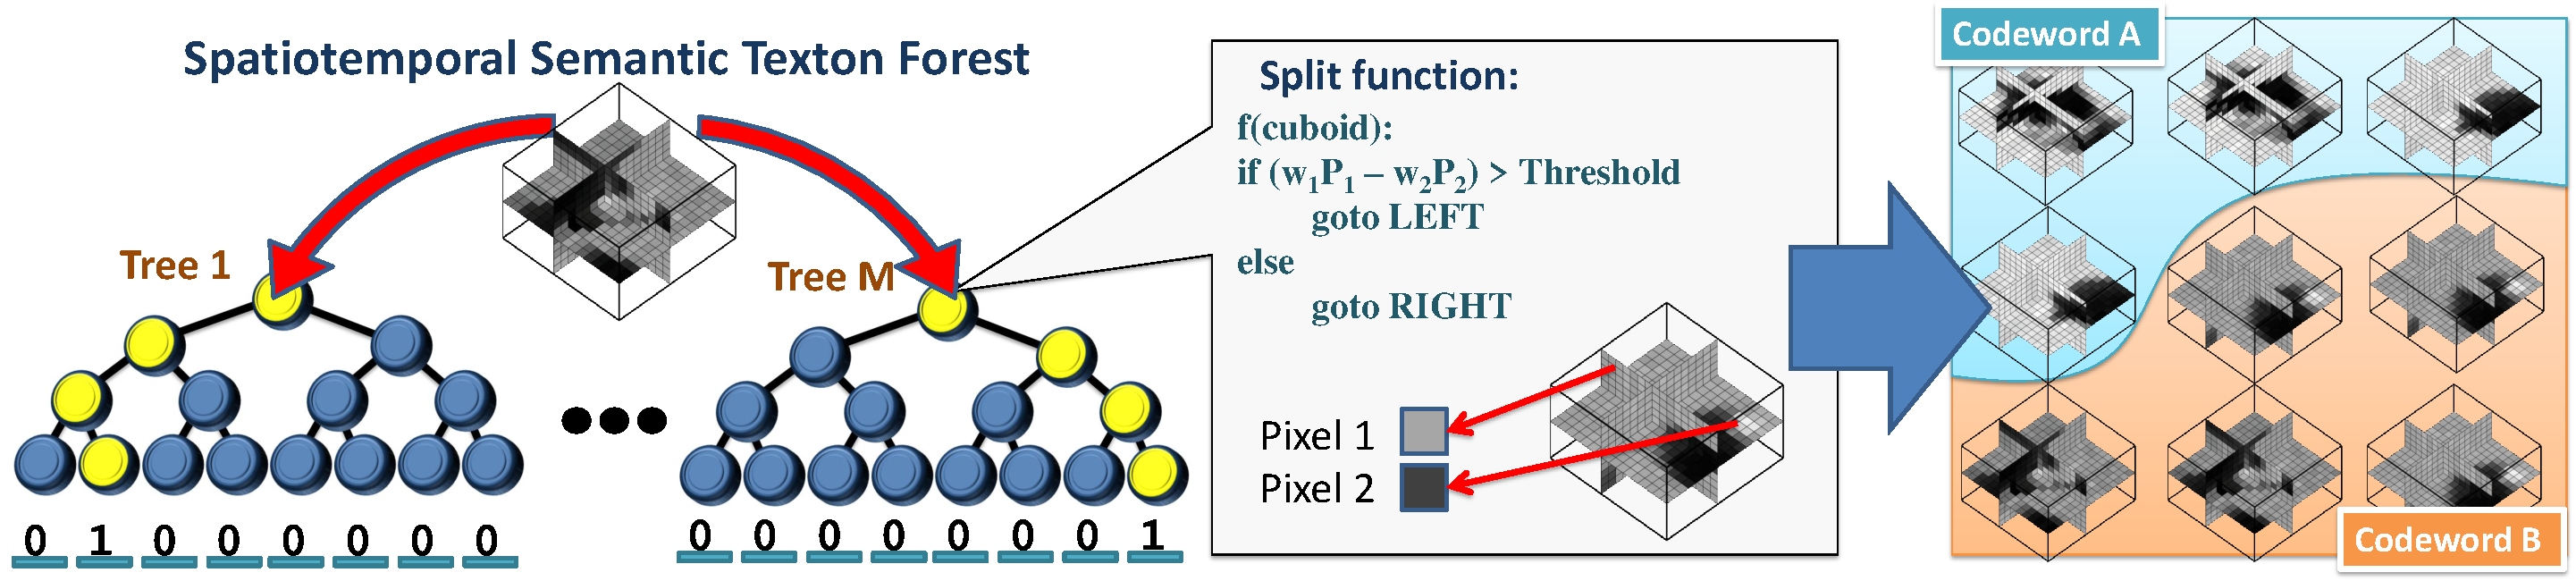
\includegraphics[width=1\linewidth]{fig/actreg/stf.pdf}%stf.png}
\caption{Visual codeword generation by Spatiotemporal Semantic Texton Forest}
\label{img:stf}
\end{figure}
Table \ref{tab:codebook} summarises a comparison between STF and k-means algorithms.
\begin{table}
\begin{center}
{\footnotesize
\begin{tabular}{|c|c|c|c|}
\hline
\textbf{ Algorithm} & \textbf{ Copmlexity} & \textbf{ Relative Speed}* & \textbf{ Hierarchical} \\
\hline
\hline
k-means & $O(K)$ & $1$ & no \\
Hierarchical k-means & $O(b\log_{b}(K))$ & $43.51$ & yes \\
{\color{blue}{STF}} & {\color{blue}{ $ O(\log_{2}(K)) $ }} & {\color{blue}{$559.86$}} & {\color{blue}{yes}}\\
\hline
\multicolumn{4}{p{0.75\linewidth}}{\scriptsize Relative speed is measured by computing $1$ million feature vectors with $405$ dimensions. Size of codebook $K$ is $1905$. The branching factor $b$ for k-means algorithm is $16$.}
\end{tabular}
}
\end{center}
\caption{Comparison of semantic texton forest and k-means codebooks.}
\label{tab:codebook}
\end{table}

\section{Multi-pyramidal Spatiotemporal Relationship Match}
\label{sec: MpSRM}
Multi-pyramidal spatiotemporal relationship match (MpSRM) is presented to encapsulate both local-appearance and structural information efficiently. Semantic texton forest quantises local space-time volumes into codewords in multiple texton trees. For each tree, a three-dimensional histogram is constructed by analysing pairs of codewords and their structural relations (see figure~\ref{img:mpsrm} (left and middle)). For each histogram, a novel pyramid match kernel is proposed for robust matching (figure~\ref{img:mpsrm} (right)). Multiple pyramidal matches are then combined to classify a query video. Whereas the spatiotemporal relationship match (SRM){Ryoo2009} relies on a single flat k-means codebook, MpSRM utilises multiple tree codebooks and pyramid match kernels. Its hierarchical structure offers a time-efficient way to perform pyramid match kernel for semantic codeword matching \cite{Grauman2005}.\vspace{-3mm}
\paragraph{Spatiotemporal relationship histograms.}
\begin{figure}
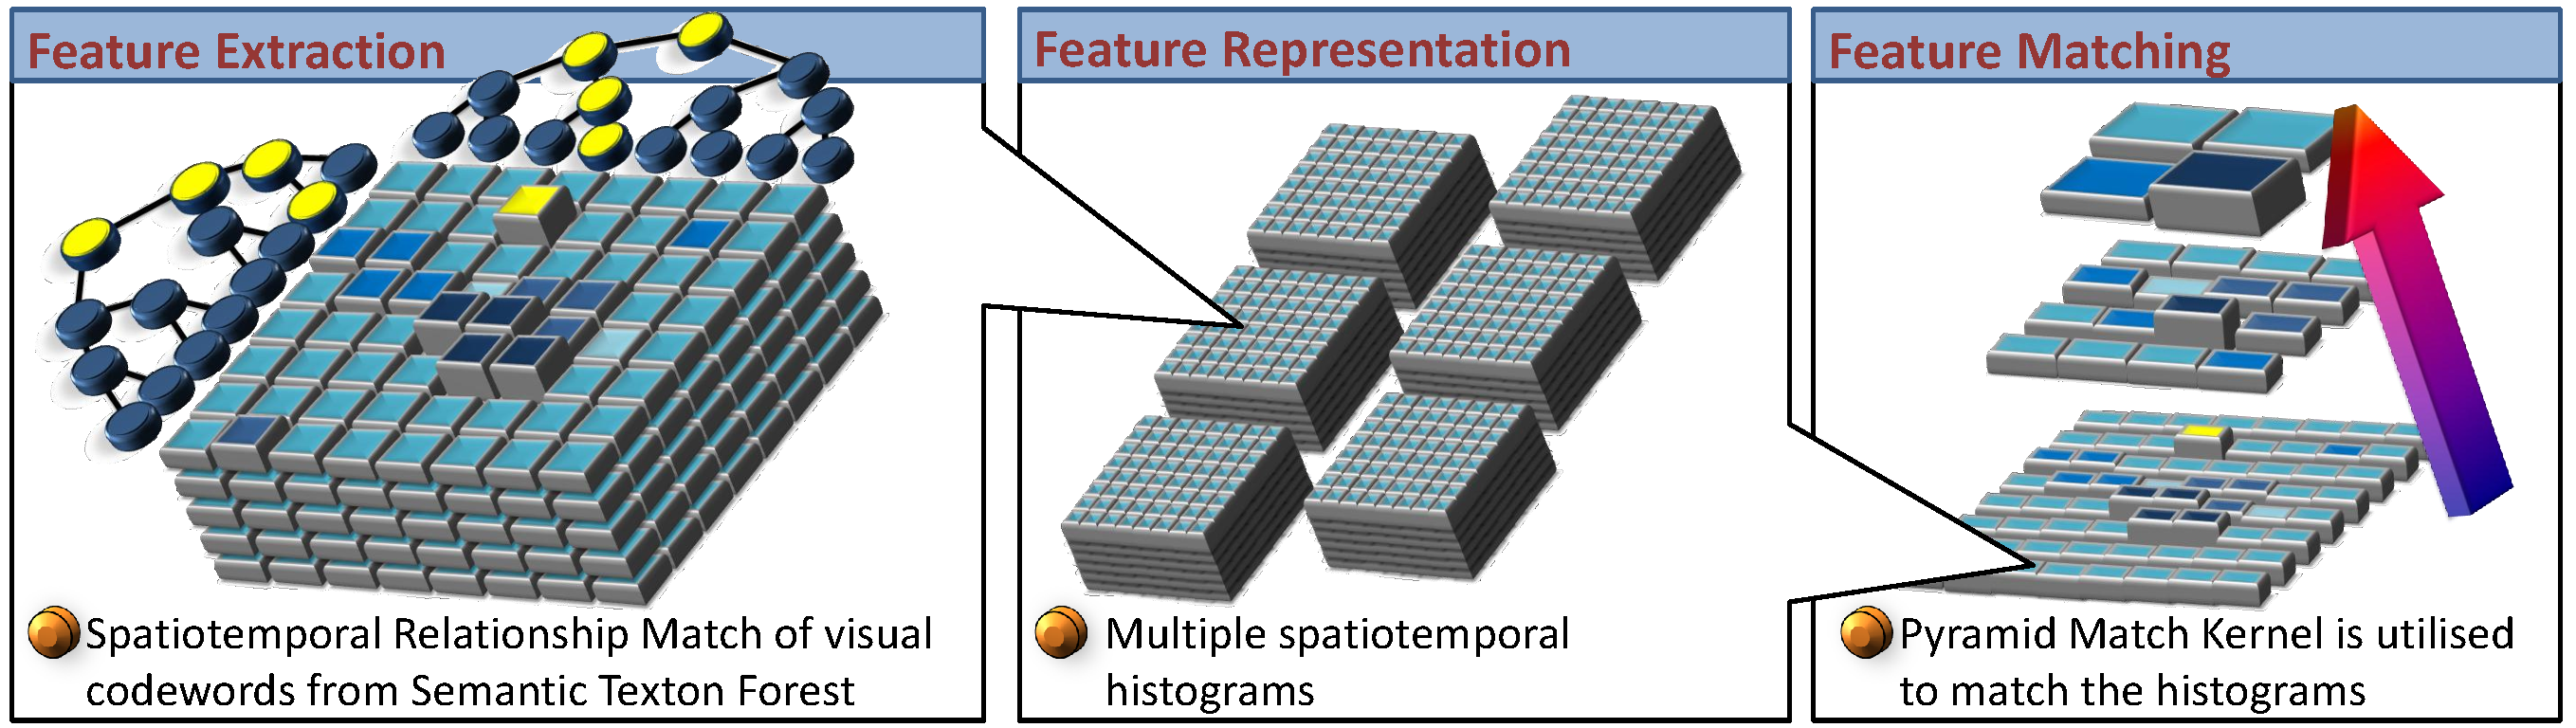
\includegraphics[width=1\linewidth]{fig/actreg/fig4.pdf}%mpsrm.png}
\caption{Multi-pyramidal spatiotemporal relationship match (MpSRM)}
\label{img:mpsrm}
\end{figure}

Short video sequences are sequentially sampled from an input video in very short intervals (\eg$10$ frames). A set of spatiotemporal interest points $\mathrm{U} = \{u_{i}\}$ are localised. The trained STF assigns visual codewords to the interest points. Therefore, an encoded interest point can be described as $u_{i} = \{x_i, y_i, t_i, l_{m,i}\}, m=1,...,M$, where $x_i, y_i, z_i$ represents a $XYT$-location of the feature and $l_{m,i}$ is the visual codeword i.e. leaf node assigned to $u_{i}$ by the $m$-th tree. A set of pair-wise spatiotemporal associations are designed to capture the structural relations among interest points. By analysing all possible pairs $u_i$ and $u_j$ in $\mathrm{U}$, space-time correlations are described by the following seven association rules $\mathrm{R} = \{ R_1,\dots,R_7\}$:

\begin{align*}%\quad ~~~
& R_{1} ~{\color{blue}overlap}: |t_i - t_j| < \mathrm{T_{o}},   & & R_{4}~{\color{blue}nearXY}: (|x_i - x_j| < \mathrm{T_{n}}) \wedge (|y_i - y_j| < \mathrm{T_{n}}) \nonumber\\
& R_{2} ~{\color{blue}before}: \mathrm{T_{o}} < t_j - t_i < \mathrm{T_{b}}, & & R_{5}~{\color{blue}nearX}: (|x_i - x_j| < \mathrm{T_{n}}) \wedge \sim(nearXY)\nonumber\\
& R_{3} ~{\color{blue}after}: \mathrm{T_{o}} < t_i - t_j < \mathrm{T_{a}}, & & R_{6}~{\color{blue}nearY}: (|y_i - y_j| < \mathrm{T_{n}}) \wedge \sim(nearXY)\nonumber\\
& R_{7} ~{\color{blue}far}: (|x_i - x_j| < \mathrm{T_{f}}) \wedge (|y_i - y_j| < \mathrm{T_{f}}) & \wedge & \sim(nearXY \vee nearX \vee nearY)
\vspace{-3mm}
\end{align*}

Figure \ref{img:mpsrm} illustrates how relationship histograms are constructed and matched in MpSRM. A set of 3D relationship histograms $\{ \mathrm{H}_1(\mathrm{U}),\dots,\mathrm{H}_{M}(\mathrm{U})\}$ are constructed by analysing the pairs of feature points in $\mathrm{U}$. The bin $\mathrm{h}_{m}(i,j,k)$ for the $m$-th tree $\mathrm{H}_{m}(\mathrm{U})$ corresponds to the number of matching $(l_{m,i},l_{m,j})$ codeword pairs by an association $R_k$. The total number of bins in $\mathrm{H}_m(\mathrm{U})$ is $L_m \times L_m \times |\mathrm{R}|$. Despite the enormous size of the relationship histograms, operations on these histograms can be greatly accelerated by using sparse matrices.

\paragraph{Pyramid match kernel for MpSRM.}
Multi-resolution matching of input features is realised by pyramid match kernel (PMK){Grauman2005}. It measures the similarity of two set of features in a multi-resolution histogram space.
The similarity between two sets of interest points $\mathrm{U}$ and $\mathrm{V}$ is measured by pyramid match kernel (PMK) from a multi-resolution histogram space for each tree. At a specific resolution $q$, the two sets $\mathrm{U}$ and $\mathrm{V}$ having the histogram bins $\mathrm{h}^q_{m}(i,j,k)$ and $\mathrm{g}^q_{m}(i,j,k)$ respectively, are matched by histogram intersection in (\ref{eq:hik}). New quantisation levels in the histogram pyramid are formed by increasing bin size. In the proposed method, adjacent bins that share the same parent node in the tree are conveniently merged in (\ref{eq:merge}), creating a new quantisation level $\mathrm{h}^{q+1}_m(i,j,k)$ (the same for $\mathrm{g}^{q+1}_m(i,j,k)$). The match kernel $\mathrm{K}_m$ for MpSRM at the $m$-th tree is then defined in (\ref{eq:pmk}) by the weighted summation of difference between successive histogram intersections. Matches in finer bins score higher similarity than matches in coarser levels by a factor of $\frac{1}{4^{q-1}}$.
\begin{eqnarray}
\label{eq:hik}
\mathrm{I}^q(\mathrm{U},\mathrm{V}) &= & \Sigma_{i=1}^{L_m}\Sigma_{j=1}^{L_m}\Sigma_{k=1}^{7} \left( \min(\mathrm{h}^{q}_m(i,j,k), \mathrm{g}^{q}_m(i,j,k)) \right)\\
\label{eq:merge}
\mathrm{h}^{q+1}_m(i,j,k) &= &\Sigma_{u=1}^{2}\Sigma_{v=1}^{2} \left( \mathrm{h}^{q}_m(2(i-1)+u,2(j-1)+v,k) \right)\\
%\label{eq:newcount}
%D^{q}_m(U,V) &= & I^q_m(U,V) - I^{q-1}_m(U,V) \\
\label{eq:pmk}
\mathrm{K}_m(\mathrm{U},\mathrm{V}) &= & \Sigma_{q = 1}^{Q}\frac{1}{4^{q-1}} \left( \mathrm{I}^{q+1}(\mathrm{U},\mathrm{V}) - \mathrm{I}^{q}(\mathrm{U},\mathrm{V}) \right)
\end{eqnarray}

\paragraph{Kenrel k-means forest classifier.}
The MpSRM is utilised to form the k-means forest classifier. Given a set of training video data $\mathrm{U}_i$, $M$ independent clustering trees are trained by recursively performing k-means algorithm on the pyramid matches. For the $m$-th tree in STF, the hierarchical k-means algorithm aims to partition the training data into $\mathbf{S}=\{S_i\}$, $i=1,...,N$ clusters so as to maximise the intra-cluster similarity by (\ref{eq:kmeans}):
\begin{equation}
\arg\max_{\mathbf{S}} \Sigma_{i = 1}^{N}\Sigma_{\mathrm{U}_j \in S_{i}} \mathrm{K}_m(\mathrm{U}_j, \mu_{m,i})
\label{eq:kmeans}
\end{equation}
where $\mu_{m,i}$ is the centroid of $i$-th cluster. In the testing stage, MpSRM is performed on a query video $\mathrm{V}$ against all centroids $\mu_{m,i}$ at the same level. The query video proceeds to the node with highest similarity score and MpSRM is performed recursively until a left node is reached. Classification is performed by the posterior probability by averaging the class distributions of the assigned leaf nodes $\{ \hat{\mu}_m \}, m=1,...,M$ trees as
\begin{equation}
\arg\max_{c}\mathrm{P}_{H}(c|\mathrm{V}) = \frac{1}{M}\Sigma_{m=1}^{M}\mathrm{P}_{H}(c|\hat{\mu}_{m})
\end{equation}

\section{Combined Classification with BOST}
\label{sec:combine}

\paragraph{Bag of semantic textons.}
The method called bag of semantic textons (BOST) developed for image classification{Shotton2008} is applied to analyse local space-time appearance. A 1-D histogram $\mathrm{B}$ is obtained by counting the occurrences of interest points at every node in the STF codebook, hence histogram size $|\mathrm{B}|$ is the total number nodes in the STF. Since its dimension $L$ is relatively low (c.f. the MpSRM histogram has $L_m \times L_m \times |\mathrm{R}|$ dimension), standard random forest \cite{Breiman2001} is applicable as a fast and powerful discriminative classifier, which has proved powerful in image categorisation and visual tracking. The random forest trained on the BOST histograms classifies a query video $\mathrm{V}$ by the posterior probability by averaging the class distributions over the assigned leaf nodes $\{\hat{l}_1,\dots,\hat{l}_{m}\}, m=1,...M$ trees in the STF: $\mathrm{P}_{B}(c|V) = \frac{1}{M}\sum_{m=1}^{M}\mathrm{P}_{B}(c|\hat{l}_m)$.

\paragraph{Combined classification.} The task of action recognition is performed separately by the proposed kernel k-means forest classifier and by the BOST method. While MpSRM has proved effective in most of the cases owing to its both local and structural information, BOST works well owing to its powerful RF classifier on some particular action classes. By integrating classification results of both methods, average performance is significantly improved. Final class label is assigned to the class $c$ which obtains the highest combined posterior probability as
\begin{equation}
\arg\max_{c}\mathrm{P}(c|\mathrm{V}) = \alpha_c \mathrm{P}_{H}(c|\mathrm{V}) + (1 - \alpha_c) P_{B}(c|\mathrm{V})
\label{eq:combine}
\end{equation}
where the weight $\alpha_c$ is selected to maximise the true positive ratio (sensitivity) of a particular class $c \in C$. Values of $\alpha_c$ are computed using gradient descent or simple line search.

\section{Experiments}
\label{sec:experiments}
The proposed method was tested on the well-known KTH data set \cite{Schuldt2004} and the UT-interaction data \cite{Ryoo2010}, a more challenging set \cite{Ryoo2009}. Other published state-of-the-art approaches are compared with the proposed method in terms of recognition accuracy. Computational time of our method is also reported. The experimental prototype was implemented in C++ on a standard PC. The system runs in real-time and makes decisions in a continuous manner (see the supplementary video submitted). 
%%%%%%%%%%%%%%%%%%%%%%%%%%%%%%%%%%%%%%%%%%%%%%%%%%%%%%%%%%%
% Example frames of KTH and UT-interaction
%%%%%%%%%%%%%%%%%%%%%%%%%%%%%%%%%%%%%%%%%%%%%%%%%%%%%%%%%%%
\begin{figure}
\centering
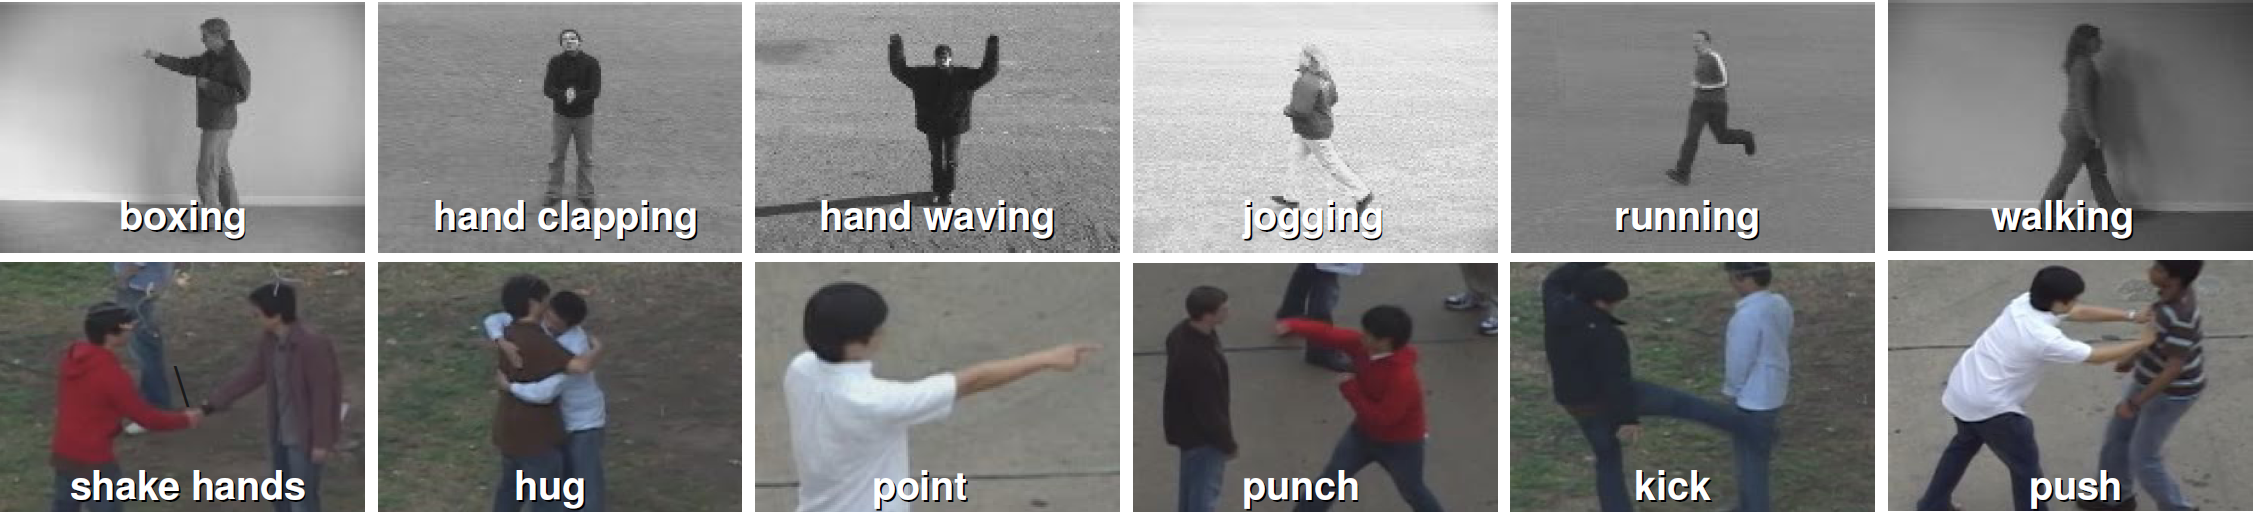
\includegraphics[width=0.8\linewidth]{fig/actreg/frames.png}
\caption{Example frames of KTH (top row) and UT-interaction (bottom row) data set}
\label{img:frames}
\end{figure}
%%%%%%%%%%%%%%%%%%%%%%%%%%%%%%%%%%%%%%%%%%%%%%%%%%%%%%%%%%%
\subsection{KTH}
% dataset introduction KTH
The KTH data set, a common benchmark for action recognition research, involves sequences of six action classes taken with camera motions, scale, appearance and subject variations (see figure~\ref{img:frames} (top)). 
%All sequences were taken at 25fps frame rate having a length of 19 seconds on average.
To demonstrate the method for continuous action recognition by a short response time, subsequences with length less than 2 seconds were extracted from the original sequences on the fly. The subsequences from training videos were used to train the classifiers. Similar subsequences were extracted from testing videos for classification. Histograms $\mathrm{B}$ and $\mathrm{H}_m(\mathrm{U})$ were computed efficiently using dynamic programming. We used leave-one-out cross validation. Most published results in the literature were reported at the sequence level, class label was assigned to the whole testing video instead of individual short subsequences. To put the proposed method in context, two different accuracies are measured: (1) ``snippet'' accuracy that is directly measured at small subsequences level; and (2) sequence level accuracy, which assigns a class label to the testing video by majority voting from subsequences' classification labels.
%%%%%%%%%%%%%%%%%%%%%%%%%%%%%%%%%%%%%%%%%%%%%%%%%%%%%%%%%%%
% Confusion matrices
%%%%%%%%%%%%%%%%%%%%%%%%%%%%%%%%%%%%%%%%%%%%%%%%%%%%%%%%%%%
\begin{figure}
\centering
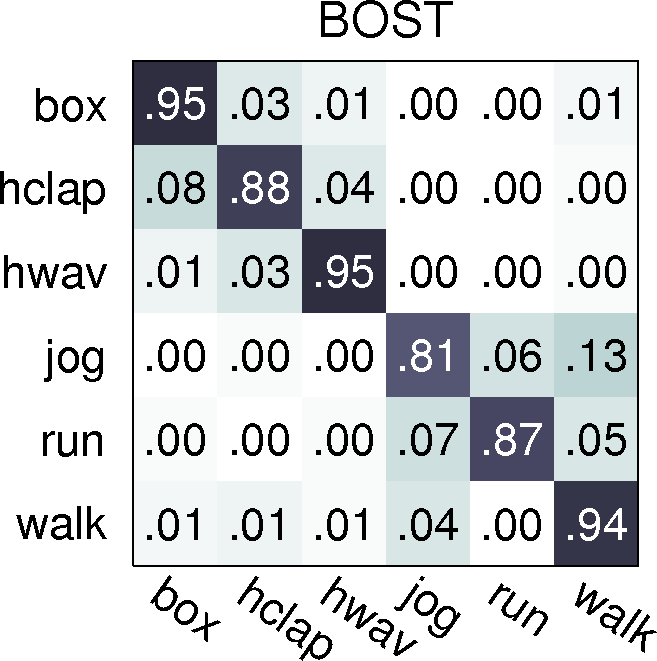
\includegraphics[width=0.2\linewidth]{fig/actreg/bost.png}
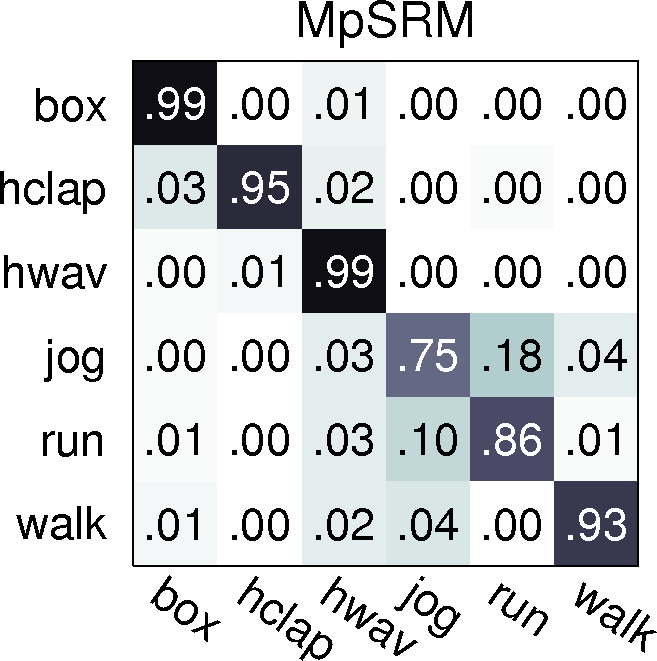
\includegraphics[width=0.2\linewidth]{fig/actreg/mpsrm.png}
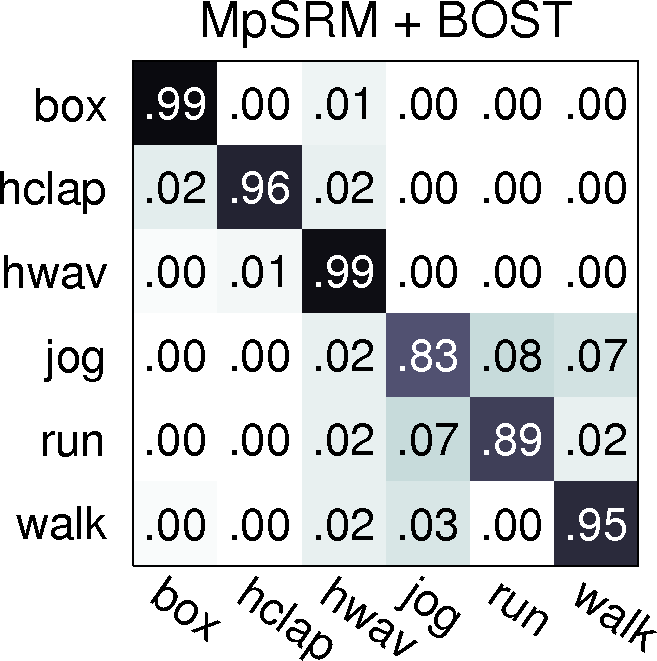
\includegraphics[width=0.2\linewidth]{fig/actreg/combine.png}
\caption{Confusion matrices of BOST (left), MpSRM (middle), and combined classification(right) on KTH dataset}
\vspace{-3mm}
\label{img:confusion}
\end{figure}
%%%%%%%%%%%%%%%%%%%%%%%%%%%%%%%%%%%%%%%%%%%%%%%%%%%%%%%%%%%
%%%%%%%%%%%%%%%%%%%%%%%%%%%%%%%%%%%%%%%%%%%%%%%%%%%%%%%%%%%
% accuracy table: KTH
%%%%%%%%%%%%%%%%%%%%%%%%%%%%%%%%%%%%%%%%%%%%%%%%%%%%%%%%%%%
\begin{table}
\centering
{\footnotesize
\begin{tabular}{|c|c|c|c|c|c|c|c|c|}
\hline
Method & box & hclp & hwav & jog & run & walk & \textbf{ Overall} & Protocol \\
\hline
\textbf{ \color{blue} MpSRM + BOST} & \textbf{ \color{blue} 100.0} & \textbf{ \color{blue}96.0} & \textbf{ \color{blue}100} & \textbf{ \color{blue}86.0} & \textbf{ \color{blue}95.0} & \textbf{ \color{blue}97.0} & \textbf{ \color{blue}95.67} & sequence\\
\textbf{ \color{blue} MpSRM + BOST} & \textbf{ \color{blue} 99.0} & \textbf{ \color{blue} 96.6} & \textbf{ \color{blue}98.9} & \textbf{ \color{blue}82.6} & \textbf{ \color{blue}89.5} & \textbf{ \color{blue}94.8} & \textbf{ \color{blue} 93.55} & snippet\\
MpSRM & 99.0 & 96.1 & 98.7 & 74.6 & 85.9 & 92.2 & \textbf{ 91.10} & snippet\\
SRM{Ryoo2009} & 96.0 & 95.0 & 97.0 & 78.0 & 85.0 & 92.0 & \textbf{ 90.5} & sequence\\
\hline
Mined features (2009) \cite{Gilbert2009} & 100.0 & 94.0 & 99.0 & 91.0 & 89.0 & 94.0 & \textbf{ 96.70} & sequence\\
CCA (2007) \cite{Kim2007} & 98.0 & 100.0 & 97.0 & 90.0 & 88.0 & 99.0 & \textbf{ 95.33} & sequence\\
Neighbourhood** (2010) \cite{Kovashka2010} & - & - & - & - & - & - & \textbf{ 94.53} & sequence\\
Info. maximisation (2008) \cite{Liu2008} & 98.0 & 94.9 & 96.0 & 89.0 & 87.0 & 100.0 & \textbf{ 94.15} & sequence\\
Shape-motion tree (2009) \cite{Lin2009} & 96.0 & 99.0 & 96.0 & 91.0 & 85.0 & 93.0 & \textbf{ 93.43} & sequence\\
Vocabulary forest (2008) \cite{Mikolajczyk2008} & 97.0 & 96.0 & 98.0 & 88.0 & 93.0 & 87.0 & \textbf{ 93.17} & sequence\\
Point Clouds (2009) \cite{Bregonzio2009} & 95.0 & 93.0 & 99.0 & 85.0 & 89.0 & 98.0 & \textbf{ 93.17} & sequence\\
pLSA-ISA (2007) \cite{Wong2007} & 96.0 & 92.0 & 83.0 & 79.0 & 54.0 & 100.0 & \textbf{ 83.92} & sequence\\
\hline
\multicolumn{9}{p{0.9\linewidth}}{\scriptsize * The length of subsequences called snippet is about 50 frames. To balance accuracy, speed and generality, the depth of random forest classifier = $8$; For k-means forest classifier: K = $10$, depth = $3$. ** Classifiers were trained by a split dataset in separate scenarios.
}\\
\end{tabular}
}
\caption{Accuracies on KTH data set by the proposed method and state-of-the-art methods. Leave one out cross validation (LOOCV) scheme was used.}
\label{tab:compare}
\end{table}
%%%%%%%%%%%%%%%%%%%%%%%%%%%%%%%%%%%%%%%%%%%%%%%%%%%%%%%%%%%

Table \ref{tab:compare} presents a detailed comparison of accuracies between our method and other state-of-the art approaches. The MpSRM+BOST model gives a very competitive accuracy, even only short subsequences are used for recognition. The confusion matrices in figure \ref{img:confusion} shows how MpSRM and BOST complement each other to attain an optimised accuracy. Quantisation effects are soothed by the multi-tree characteristics and pyramid matching of the proposed method, compared to the original Spatiotemporal Relationship Match method{Ryoo2009}.

Table \ref{tab:speed} summarises the experiment results on recognition speed. Different from other sequence-level recognition approaches, a more realistic metric is designed to measure the algorithm efficiency. All recognition stages (including feature detection, feature extraction and classification) are timed, and the average speed is defined as $(\mbox{\textit{ total number of subsequences}})/$ $(\mbox{\textit{ total recognition time}})$ \textbf{FPS}. It shows that the proposed method runs at 10 to 20 frames per second. The introduction of STF has greatly improved the speed for feature extraction and codeword generation, outperforming the k-means visual codebooks (see also Table~\ref{tab:codebook}). Using random forest and kernel k-means forest has provided faster solutions to match and classify multi-dimensional histograms over the traditional nearest neighbour and SVM. 
%%%%%%%%%%%%%%%%%%%%%%%%%%%%%%%%%%%%%%%%%%%%%%%%%%%%%%%%%%%
% Speed table
%%%%%%%%%%%%%%%%%%%%%%%%%%%%%%%%%%%%%%%%%%%%%%%%%%%%%%%%%%%
\begin{table}
\centering
{\footnotesize
\begin{tabular}{|c|c|c|c|c|c|c|}
\hline
Dataset & V-FAST  & STF and BOST & MpSRM & Random & k-means & \textbf{ Total }\\
 & feature detection &   &  & forest & forest & \textbf{ FPS}\\
\hline
KTH & 66.1 & 59.3 & 194.17 & 1137.6 & 67.1 & \textbf{ 18.98 } \\
UT-interaction & 35.1 & 25.8 & 35.1 & 612.2 & 428.1 & \textbf{ 10.02 } \\
\hline
\end{tabular}
}
\caption{A list of the average recognition speed at different stages in frame per second (FPS)}
\label{tab:speed}
\end{table}
%%%%%%%%%%%%%%%%%%%%%%%%%%%%%%%%%%%%%%%%%%%%%%%%%%%%%%%%%%%
%%%%%%%%%%%%%%%%%%%%%%%%%%%%%%%%%%%%%%%%%%%%%%%%%%%%%%%%%%%
% accuracy table: UT-interaction
%%%%%%%%%%%%%%%%%%%%%%%%%%%%%%%%%%%%%%%%%%%%%%%%%%%%%%%%%%%
\begin{table}
\centering
{\footnotesize
\begin{tabular}{|c|c|c|c|c|c|c|c|c|}
\hline
Method & shake & hug & point & punch & kick & push & \textbf{ Overall} & Protocol \\
\hline
\textbf{ \color{blue} MpSRM+BOST} & \textbf{ \color{blue} 100.0} & \textbf{ \color{blue}65.0} & \textbf{ \color{blue}100.0} & \textbf{ \color{blue}85.0} & \textbf{ \color{blue}75.0} & \textbf{ \color{blue}75.0} & \textbf{ \color{blue}83.33} & sequence\\
MpSRM & 90.0 & 50.0 & 85.0 & 65.0 & 70.0 & 40.0 & \textbf{ 66.67} & sequence\\
BOST & 80.0 & 50.0 & 100.0 & 65.0 & 25.0 & 35.0 & \textbf{ 59.16} & sequence\\
\hline
*SRM{Ryoo2009} & 75.0 & 87.5 & 62.5 & 50.0 & 75.0 & 75.0 & \textbf{ 70.8} & sequence\\
\hline
\multicolumn{9}{p{0.9\linewidth}}{\scriptsize * An unsegmented UT-interaction dataset was used in the experiments}\\
\end{tabular}
}
\caption{Accuracies on UT-interaction dataset. Leave one out cross validation (LOOCV) scheme were used.}
\label{tab:utcompare}
\end{table}
%%%%%%%%%%%%%%%%%%%%%%%%%%%%%%%%%%%%%%%%%%%%%%%%%%%%%%%%%%%
\subsection{UT-interaction Data set}
% dataset introduction UT
The UT-interaction data set contains six classes of realistic human-human interactions, including shaking hands, pointing, hugging, pushing, kicking and punching (see figure~\ref{img:frames} (bottom)). Some challenging factors of this data set include moving background, cluttered scene, camera jitters/zoom and different clothing. In the experiments, the segmented UT-interaction data set was used for evaluating the recognition accuracy and speed of our method. As reported in table \ref{tab:utcompare}, the proposed method marked the best accuracy in recognising challenging realistic human-human interactions. Under complex human interactions, MpSRM using both local-appearance and structural cues appeared to be more stable than BOST that uses only local-appearance. However, there still exist improvements in overall recognition accuracies in the combined approach. The method runs at high speed more than 10 frames per second from table \ref{tab:speed}. The recognition speed on this data set over KTH has dropped due to extra interest points from other moving objects in the scene.

\section{Conclusion}
\label{sec:discussion}
%advantages: fast, fully utilises structural information
%limitation: still have some lookahead, not so powerful features, localisation not optimised
This paper has presented a novel solution for action recognition. Different from other published approaches, a major strength of our method is the run-time speed. Real-time performance is achieved by semantic texton forest which works on video pixels generating visual codewords in an extremely fast manner. MpSRM is proposed to capture both spatiotemporal structures and local-appearances of actions and ease quantisation effects based on STF. Furthermore, a novel fast interest point detector and application of random forest and kernel k-means forest classifiers contribute to the acceleration of recognition speed. Experimental results show the comparable accuracies of the proposed method compared to state-of-the-arts. A future challenge will be tackling more complex realistic human actions and partial occlusions, as well as requiring continuous action localisation with a real-time performance.

